\documentclass[10pt,a4paper]{article}
\usepackage[utf8]{inputenc}
\usepackage{graphicx}
\usepackage{pdfpages}
\author{renatolrr}
\title{Polarización universal o por divisor de tensión}
\begin{document}
\maketitle
Vamos a calcular el siguiente circuito:

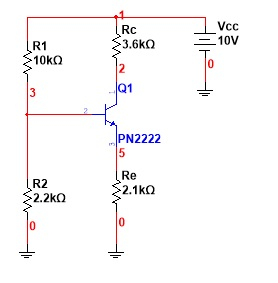
\includegraphics[scale=1]{Images/Imagen1.jpg} 

Para el análisis sustituimos el divisor resistivo por el equivalente de Thevénin entre la base y la masa.

\section{Equivalente Thévenin}
\subsection{Calculo de $R_{0}$}
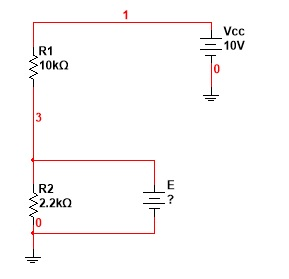
\includegraphics[scale=1]{Images/Imagen2.jpg}
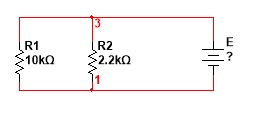
\includegraphics[scale=1]{Images/Imagen3.jpg} 
\\
Con Vcc en corto tenemos que calcular Ro
\[R=E/I\]
Si nos fijamos son las dos resistencias en paralelo, luego la resistencia equivalente es:
\[R_{0}=\frac{R_{1}*R_{2}}{R_{1}+R_{2}}\]
Por lo tanto tenemos en nuestro caso:
\[R_{0}=R_bb=\frac{10K*2.2k}{10K+2.2K}\]
\subsection{Calculo de $E_{0}$}
La intensidad de base es cero por lo tanto tenemos:
\begin{center}
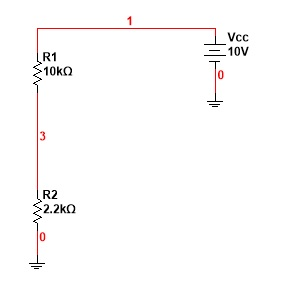
\includegraphics[scale=1]{Images/Imagen4.jpg}
\end{center}
Y calculamos $E_{0}$
\[E_{o}=\frac{V_{cc}}{R_{1}+R_{2}}*R_{2}\]
En nuestro caso 
\[E_{o}=V_{bb}=\frac{10V}{10K+2.2K}*2.2K=1.8V\]
\subsection{Circuito equivalente}
A partir de este momento utilizamos el circuito equivalente:
\\
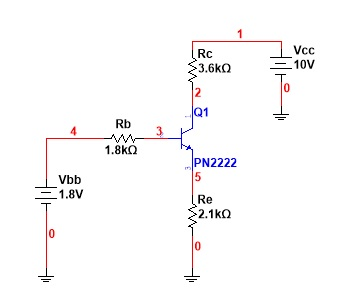
\includegraphics[scale=1]{Images/Imagen5.jpg}
\section{Valores de la intensidad y del voltaje}
\subsection{Ecuaciones fundamentales}
\begin{equation}
I_{e}=I_{c}+I_{b}
\end{equation}
\begin{equation}
I_{c}=\beta*I_{b}
\end{equation}
\subsection{Malla base}
Si consideramos la malla base tenemos:
\begin{center}
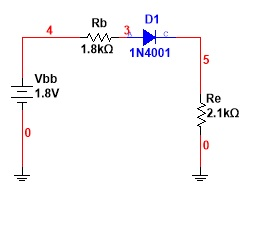
\includegraphics[scale=1]{Images/Imagen6.jpg}
\end{center}
Luego se tiene:
\begin{equation}
V_{bb}=I_{b}R_{b}+V_{be}+I_{e}R_{e}
\end{equation}
Vamos a calcular $I_{b}$ y para ello utilizamos las ecuaciones (1) y (2):
\[I_{e}=I_{b}+I_{c}\]
\[\Rightarrow I_{e}=I_{b}+\beta*I_{b}\]
\[\Rightarrow I_{e}=I_{b}(\beta+1)\]
Si lo sustituimos en la ecuación (3) se tiene:
\[V_{bb}=I_{b}R_{b}+V_{be}+I_{e}R_{e}\]
\[\Rightarrow V_{bb}=I_{b}R_{b}+V_{be}+I_{b}(\beta+1)R_{e}\]
\[\Rightarrow V_{bb}=I_{b}[R_{b}+(\beta+1)R_{e}]+V_{be}\]
y despejando se tiene:
\[I_{b}=\frac{V_{bb}-V_{be}}{[R_{b}+(\beta+1)R_{e}]}\]
Y si sustituimos nuestros valores:
\[I_{b}=\frac{1.8V-0.7V}{[1.8K+(100+1)2.1K]}=5.142 \mu A\]
Ojo: $V_{be}=0.7V$ ya que tenemos el diodo del transistor.
\\ 
Ya podemos calcular $I_{c}$ a partir de la ecuación (2) que en nuestro caso nos da:
\[I_{c}=\beta*I_{b}\]
\[I_{c}=100*5.142 \mu A= 0.514 mA\]
Y  con la ecuación (1) tenemos $I_{e}$ que en nuestro caso:
\[I_{e}=I_{b}+I_{c}\]
\[I_{e}=0.519 mA\]
Podemos decir que $I_{CQ}=0.514 mA$
\subsection{Malla colector}
\begin{center}
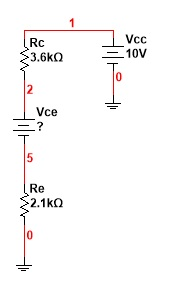
\includegraphics[scale=1]{Images/Imagen7.jpg}
\end{center}
Y la ecuación correspondiente es:
\begin{equation}
V_{cc}=I_{c}R_{c}+V_{ce}+I_{e}R_{e}
\end{equation}
Vamos a calcular $V_{ce}$ :
\[V_{cc}=I_{c}R_{c}+V_{ce}+I_{e}R_{e}\]
\[\Rightarrow V_{ce}= V_{cc}-I_{c}R_{c}-I_{e}R_{e}\]
Y si lo sustituimos en nuestro caso:
\[V_{ce}= 10V-0.5141mA-0.519mA*2.1K= 7.06V\]
Y podemos decir que $V_{CEQ}=7V$
\section{Recta de carga}
\subsection{Demostrar que la Ie es igual a Ic para ganancias muy grandes}
De la ecuación (2) se tiene:
\[I_{b}=\frac{I_{b}}{\beta}\]
Y sustituyendo en (1):
\[I_{e}=I_{c}+I_{b}\]
\[\Rightarrow I_{e}=I_{c}+\frac{I_{b}}{\beta}\]
\[\Rightarrow I_{e}=I_{c}*(\frac{1}{\beta}+1)\]
\[\Rightarrow I_{e}=I_{c}*(\frac{\beta+1}{\beta})\]
Y si $\beta$ es muy grande:
\[I_{e}\simeq I_{c}\] 
\subsection{Calculo de la ecuación de la recta de carga}
Si $\beta$ es muy grande, tenemos $I_{e}\simeq I_{c}$ 
\\
Y de la malla del colector (Punto 2) teníamos la ecuación (4):
\[V_{cc}=I_{c}R_{c}+V_{ce}+I_{e}R_{e}\]
\begin{equation}
\Rightarrow V_{cc}=V_{ce}+I_{c}(R_{c}*R_{e})
\end{equation}
\subsection{Corte con los ejes}
\subsubsection{Punto corte eje vertical}
Hacemos $V_{ce}=0$ y de  la ecuación (5) se tiene:
\[V_{cc}=I_{c}(R_{c}*R_{e})\]
\[\Rightarrow I_{c}=\frac{V_{cc}}{R_{c}*R_{e}}\]
y en nuestro caso:
\[V_{cc}=I_{c}(R_{c}*R_{e})\]
\[I_{c}=\frac{10V}{3.6k*2.1k} = 1.754 mA \]
\subsubsection{Punto corte eje horizontal}
Hacemos $I_{c}=0$ y de  la ecuación (5) se tiene:
\[V_{cc}=V_{ce}\]
y en nuestro caso:
\[V_{ce}=10V\]
\subsection{Representación gráfica recta de carga del circuito}
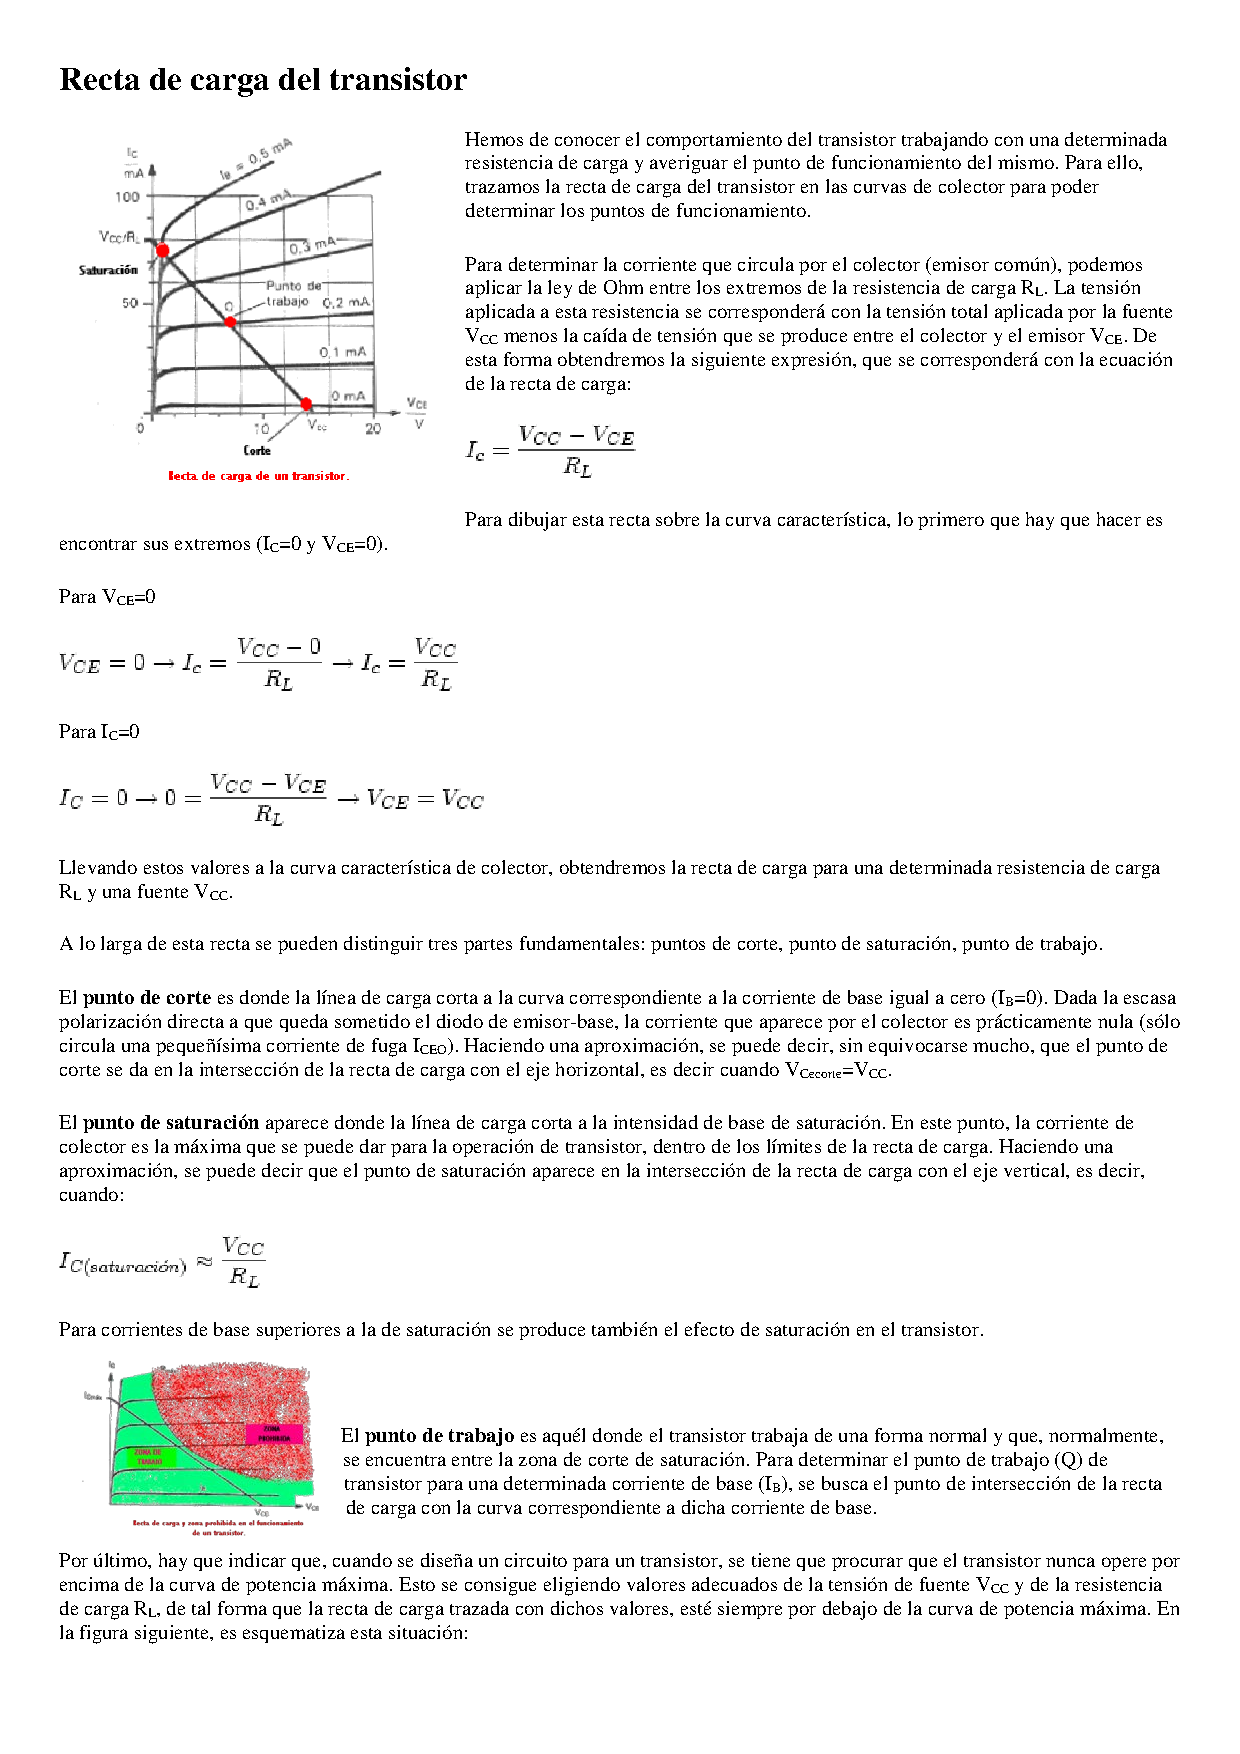
\includepdf[pages=-]{Images/RectaCarga}
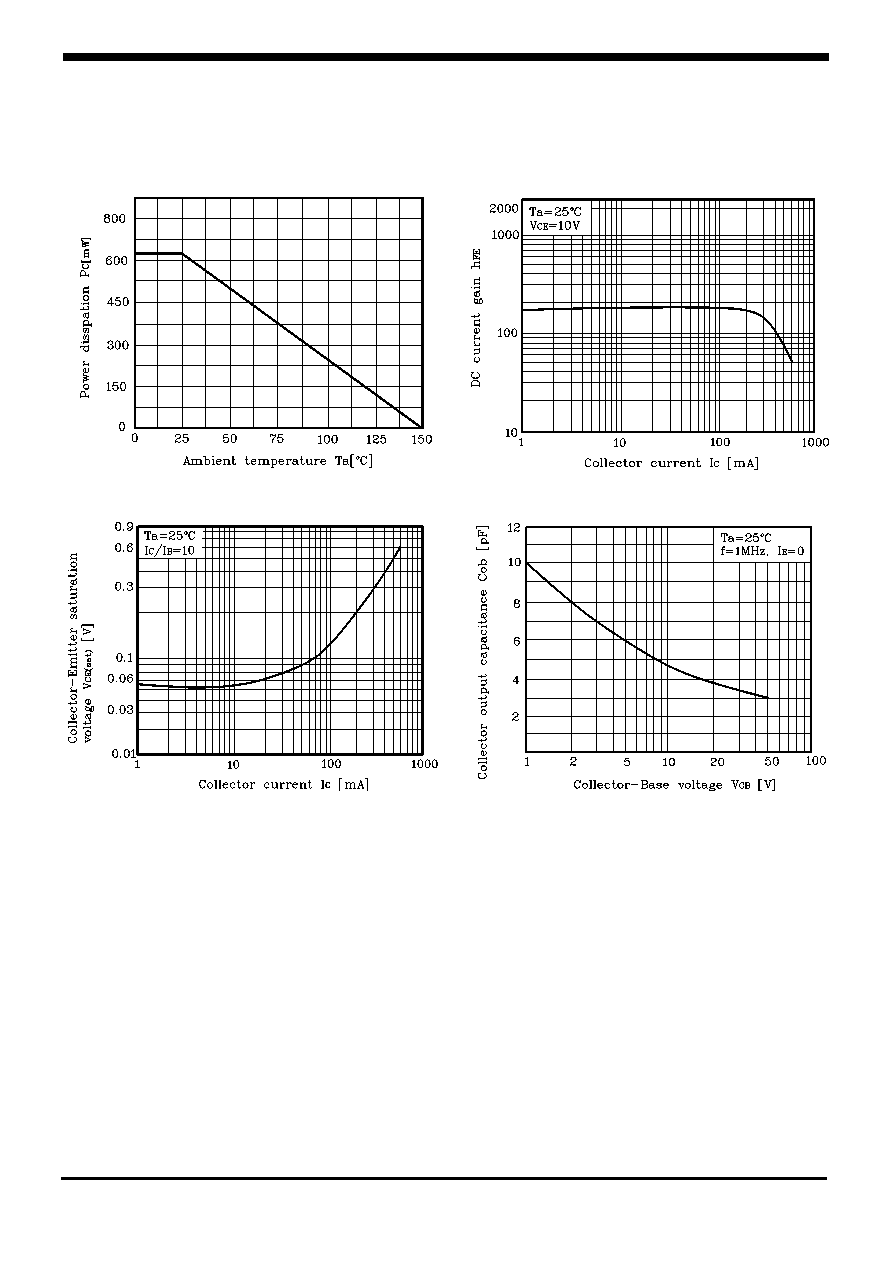
\includegraphics[scale=1]{Images/PN2222.png}
\end{document}
